%!TEX root = ../thesis.tex
%*******************************************************************************
%****************************** Third Chapter **********************************
%*******************************************************************************
\chapter{Sparsification Lemma} \label{chap:sparsication}

% **************************** Define Graphics Path **************************
\ifpdf
    \graphicspath{{Chapter4/Figs/Raster/}{Chapter4/Figs/PDF/}{Chapter4/Figs/}}
\else
    \graphicspath{{Chapter4/Figs/Vector/}{Chapte4/Figs/}}
\fi



\section*{Introduction}
% State how it would be used
In this chapter we will explain the sparsification lemma that allowed
us to show lower bounds on problems in $P$ conditioned on the SETH in Chapter \ref{chap:complexity}.
To do this we will first consider an example problem which again motivates the need
for the sparsification lemma. The example is the following.
Recall the definition of $s_k$ from Equation \ref{eq:ETH}.
\begin{theorem}
    If there exists a $k \geq 3$ such that $s_k > 0$, then $s_3 > 0$ \cite{impagliazzo2001complexity}.
\end{theorem}
To show this, we would have to prove that if there are no subexponential
time algorithms for $k$-SAT for some $k > 3$ then there is no subexponential algorithm for 3-SAT.
To make things simpler, we will show the contrapositive, that if there is a subexponential time algorithm
for 3-SAT then there is a subexponential time algorithm for $k$-SAT for all $k \geq 3$.

Assume then that we have an algorithm $A$ that solves 3-SAT in subexponential time
i.e. it takes $\mathcal{O}^{\ast}(2^{\epsilon n})$ time and we want to solve an
instance of $k$-SAT where $k > 3$. We can attempt to solve this
instance via a reduction to 3-SAT.
To reduce k-SAT to 3-SAT consider a k-CNF formula $F_{k}$ and consider a specific clause
$C = (x_{1} \lor x_{2} \lor \ldots \lor x_{k})$ from $F_k$. We will then introduce new variables
$y_{1}, y_{2}, \ldots, y_{k-3}$ and define $k-2$ new clauses as follows:

\begin{align*}
C'_{1} &= (x_{1} \lor x_{2} \lor y_{1}) \\
C'_{2} &= (\overline{y_{1}} \lor x_{3} \lor y_{2}) \\
C'_{3} &= (\overline{y_{2}} \lor x_{4} \lor y_{3}) \\
&\hspace{30pt}\vdots \\
C'_{k-2} &= (\overline{y_{k-3}} \lor x_{k-1} \lor x_{k})
\end{align*}

Observe that the conjunction of the clauses $C'_{1}, C'_{2}, \dots, C'_{k-2}$
is satisfiable if and only if the original clause $C$ is satisfiable.
This procedure can then be repeated for all clauses in $F_{k}$ to convert
the $k$-SAT formula with $n$ variables and $m$ clauses to a 3-SAT formula with $n + (k-3)m$ variables
and $(k-2)m$ clauses.
If we now use algorithm $A$, then we solve the instance in time $\mathcal{O}^{\ast}(2^{\epsilon \cdot (n + (k - 3)m)})$.
This is an issue, if we consider the fact that for an arbitrary $k$-SAT formula the number of
clauses could be significantly larger than the number of variables. Consider the case where $m = n^2$.
This then means that $A$ would run in time $2^{\mathcal{O}(n^2)}$ which is certainly not subexponential.

Fundamentally, the issue is that the reduction introduced too many new variables and these new variables
came from the number of clauses in the original formula. If we could guarantee that the number of
clauses in original formula was linear in the number of variables, i.e. $m = \mathcal{O}(n)$,
then the reduction would work.

\section{Statement of the lemma}
% State the lemma
The sparsification lemma as stated by Impagliazzo, Paturi and Zane originally relates to
$k$-Set Cover, from which they derive the k-SAT version as a corollary \cite{impagliazzo2001problems}.
The original formulation is stated here for completeness. Note that although this problem is called
$k$-Set Cover by Impagliazzo et al. \cite{impagliazzo2001problems}, it is typically refered to as $k$-Hitting Set.

An instance of $k$-Set Cover has a universe of $n$ elements $x_1, x_2, \dots, x_n$ and a collection $\mathcal{S}$
of subsets $S \subseteq \{x_1, x_2, \dots, x_n\}$. However, $\forall S \in \mathcal{S} : |S| \leq k$.
A $k$-set cover is a set $C \subseteq \{x_1, x_2, \dots, x_n\}$ such that $\forall S \in \mathcal{S} : S \cap C \neq \emptyset$.
Let $\sigma(\mathcal{S})$ be the collection of all such sets that cover $\mathcal{S}$. The goal is to find a minimal size $k$-set cover.
Let $\mathcal{T}$ be a restriction on $\mathcal{S}$ if for each $S \in \mathcal{S}$ there is a $T \in \mathcal{T}$ such that $T \subseteq S$.

\begin{theorem} \label{thm:kset_sparse}
    (Sparsification Lemma for $k$-Set Cover)
    For all $\epsilon > 0$ and $k \in \mathbb{N}^{+}$ there is a constant $C$ and an algorithm that given an instance $\mathcal{S}$
    of $k$-Set Cover on a universe of size n, produced a list of $t \leq 2^{\epsilon n}$ restrictions $\mathcal{T}_1, \mathcal{T}_2, \dots, \mathcal{T}_t$
    of $\mathcal{S}$ so that $\sigma(\mathcal{S}) = \bigcup_{i = 1}^{t} \sigma(\mathcal{T}_i)$ and so that $\forall i: |\mathcal{T}_i| \leq Cn$.
    Additionally the algorithm runs in time $\mathcal{O}^{\ast}(2^{\epsilon n})$ \cite{impagliazzo2001problems}.
\end{theorem}

This essentially states that for each $k$ and $\epsilon$ there exists an algorithm that can compute a subexponential number
of new collections such that each new collection contains a number of subsets linear in $n$.
The corollary for k-SAT can be obtained by considering the universe of elements in $k$-Set Cover to be
the $2n$ literals in the formula. $\mathcal{S}$ is then the formula with each $S \in \mathcal{S}$ being a clause.
We also require an additional set for each variable, $\{x_i, \overline{x_i}\}$, thus every cover of size exactly $n$
covers exactly one literal for each variable. Each restriction $\mathcal{T}_i$ can be thought of as a subformula of $\mathcal{S}$.

\begin{corollary} \label{cor:ksat_sparse}
    (Sparsification Lemma for $k$-SAT)
    For all $k \in \mathbb{N}^{+}$ and $\epsilon > 0$ there exists an algorithm that takes in a $k$-CNF formula $F$
    with $n$ variables and $m$ clauses and returns a collection of $k$-CNF formulas 
    $F'_1, F'_2, \dots, F'_t$, with the following properties.
    \begin{enumerate}
        \item $F$ is satisfiable if and only if $\bigvee_{i=1}^{t} F'_i$ is satisfiable.
        \item $F'_i$ has no more variables than $F$
        \item Number of clauses in $F'_i$ is less than $c(k, \epsilon)n$, where $c(k, \epsilon)$
        is a constant that does not depend on $n$.
        \item The algorithm takes time $\mathcal{O}^{\ast}(2^{\epsilon n})$ and $t \leq 2^{\epsilon n}$
    \end{enumerate}
\end{corollary}

To see how this could be used, consider the issue from earlier.
Recall that we had an instance of $k$-SAT $F$ with $m = n^2$.
After a reduction to 3-SAT this instance could be solved in time $2^{\mathcal{O}(n^2)}$.
Consider first applying the lemma $F'_1, F'_2, \dots, F'_t = \texttt{Sparsify}(F, \epsilon_2)$ for some $\epsilon_2 > 0$.
Apply the reduction to each $F'$ and solve them with the subexponential algorithm for 3-SAT.
Since, by the lemma, the number of clauses in each $F'_i$ is linear in $n$ we get that the time to solve a single
instance after the reduction to 3-SAT is $\mathcal{O}^{\ast}(2^{\epsilon_1 \cdot (n + (k-3)c(k, \epsilon_2)n )})$, 
where $\epsilon_1$ is the $\epsilon$ that we choose for our subexponential time algorithm for 3-SAT.
Choosing $\epsilon_1 > 0$ small enough we can eliminate the other constants to show that
a single $F'_i$ can be solved in time $\mathcal{O}^{\ast}(2^{\epsilon_3 n})$
for any $\epsilon_3 > 0$.
Sparsification can be done in time $\mathcal{O}^{\ast}(2^{\epsilon_2 n})$, the reduction to 3-SAT takes polynomial time.
Hence the total time is
\begin{equation} \label{eq:run_time}
    \mathcal{O}^{\ast}(2^{\epsilon_2 n}) + 2^{\epsilon_2 n} \cdot poly(n) \cdot \mathcal{O}^{\ast}(2^{\epsilon_3 n})
\end{equation}
By choosing constants $\epsilon_2$ and $\epsilon_3$ this can be simplified
to $\mathcal{O}^{\ast}(2^{\epsilon n})$ for any $\epsilon > 0$. So we can solve $k$-SAT in subexponential time
which is what we wanted to show.
Hence, what remains is to detail the sparsification algorithm and to prove the sparsification lemma.

% clean up notation wrt polynomial factors

\section{The Sparsification Algorithm}
\subsection{Flowers}
% Define some notation (formula as a set, clauses as a set, vars and lits as a function)
Before moving forward, it makes sense to define some new notation which will
be helpful later. This notation borrows from the $k$-Set Cover formulation of the
Sparsification Lemma. We will consider a Formula $F$ with $n$ variables and $m$ clauses
as a set of clauses $\{C_1, C_2, \dots, C_m\}$
with each $C$ being a set of literals $\{l_1, l_2, \dots, l_s\}$ 
with a literal being either a variable or its negation and $|C| \leq k$.
Let $$vars(F) = \{x \hspace{3pt} : x \in C \lor \neg x \in C, C \in F\}$$
and let $lits(F) = \bigcup_{C \in F}C$. It is then easy
to see that $|F| = m$ and $|vars(F)| = n$.

We can now being to describe the workings of the algorithm. Let the constants
$k$ and $\epsilon > 0$ be given. Define a sequence of $\theta_1, \theta_2, \dots, \theta_k$.
Their values will be decided at a later point
and will depend \textit{only} on k and our choice of $\epsilon$
but for now consider $\theta_i$ to be much larger than $\theta_{i-1}$.

% Descriptions of flowers (and maybe a nice diagram)
% What makes a good flower
\begin{definition}
    (Flower) A flower is a set of clauses $G = \{C_1, C_2, \dots, C_t\}$ with the following properties:
    \begin{enumerate}
        \item $\exists l \in \mathbb{N}: \forall C \in G: |C| = l$. All clauses have the same size $l$.
        \item $H = \bigcap_{C \in G} C \neq \emptyset$. The intersection of the clauses is non-empty.
    \end{enumerate}
    Denote $H = \bigcap_{C \in G} C$ as the heart and $P_i = C_i \setminus H$ as the petals. A flower
    is considered good if it has many short petals. More formally a flower is good if and only if
    \begin{equation} \label{eq:good_flower}
        |G| \geq \theta_{l - |H|}
    \end{equation}
\end{definition}

Of good flowers $G_1$ and $G_2$, we say that $G_1$ is better than $G_2$ if it has shorter clauses
$l_1 < l_2$ or if $l_1 = l_2$ but $|H_1| > |H_2|$.
It is worth noting that all of these intersections are over literals, so $\{x\} \cap \{\neg x\} = \emptyset$.

\begin{example}
    We can consider a simple formula
    \begin{align*}
    F = &\{C_1, C_2, C_3, C_4, C_5\} \\
    F = \{ &\{w, x, y, z\}, \{w, \neg x, y, \neg z\}, \{\neg w, \neg x, \neg y, \neg z\} \\
    &\{\neg w, x, y, z\}, \{\neg w, x, y, \neg z\} \}
    \end{align*}
    We can form a flower with $G = \{C_1, C_2, C_4, C_5\}$, such that the heart $H = \{y\}$
    and the petals $P = \{\{w, x, z\}, \{w \neg x, \neg z\}, \{\neg w, x, z\}, \{\neg w, x, \neg z\}\}$.
    Note that in this case $l = 4$ and for the flower to be good we would need to satisfy equation 
    \ref{eq:good_flower}, so we must have $|G| \geq \theta_{4 - |H|}$ or $5 \geq \theta_{3}$.
    This flower can be seen in Figure \ref{eq:good_flower}.
\end{example}

\begin{figure}
    \centering
    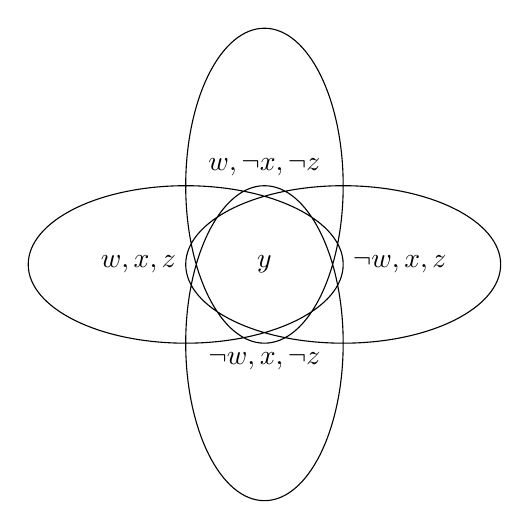
\begin{tikzpicture}
        \draw[] (-1,0) ellipse (2 and 1) node[anchor=east]{$w, x, z$}
                (0,1) ellipse (1 and 2) node[anchor=south]{$w, \neg x, \neg z$}
                (1,0) ellipse (2 and 1) node[anchor=west]{$\neg w, x, z$}
                (0,-1) ellipse (1 and 2) node[anchor=north]{$\neg w, x, \neg z$};
        \node (0,0) {$y$};
    \end{tikzpicture}
    \caption{Visualisation of a flower with 4 petals and $H = \{y\}$.}
    \label{fig:flower}
\end{figure}

\subsection{Algorithm}
% Describe the recursive algorithm
The Sparsification Algorithm at each step finds the best flower and then adds
the petals to one copy of the formula and the heart to the other copy of the formula,
removing redundant clauses. The algorithm then applies itself recursively to the two
new formulas. If there are no good flowers, then we are done. This algorithm can
be seen in Algorithm \ref{alg:sparse}.

\begin{algorithm}
\caption{Sparsification Algorithm (\texttt{sparsify})}
\label{alg:sparse}
\vspace{5pt}
\KwIn{$k$-CNF Formula $F$, $k \in \mathbb{N}$, $\epsilon > 0$}
\KwOut{$F'_1, F'_2, \dots, F'_t$}
\hrulefill\\

\nl $G = \{C_1, C_2, \dots C_s\} \gets \texttt{best\_flower}(F, \epsilon, k)$ \\
\nl \If{$F$ contains a good flower}{
    \nl $H \gets \bigcap_{C \in G}C$ \\
    \nl $P \gets \{C \setminus H : C \in G\}$ \\
    \nl $F_{\textit{heart}} \gets \texttt{reduce}(F \cup \{H\})$ \\
    \nl $F_{\textit{petals}} \gets \texttt{reduce}(F \cup P)$ \\
    \nl \Return{ }$\texttt{sparsify}(F_{\textit{heart}}, k, \epsilon) \cup$ \\ 
    $\hspace{30pt} \texttt{sparsify}(F_{\textit{petals}}, k, \epsilon)$ \\
}
\nl \Else{
    \nl \Return{$F$}
}
\end{algorithm}

\begin{figure}
    \centering
    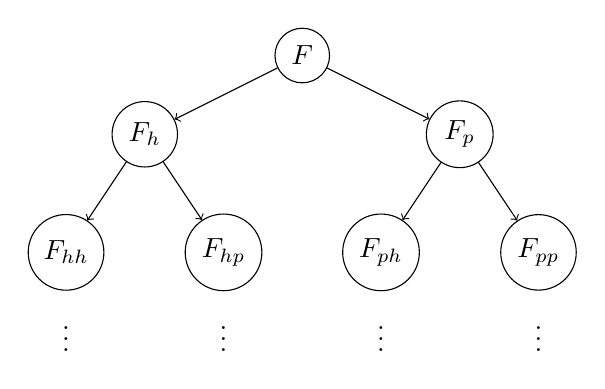
\begin{tikzpicture}
        \node[draw, circle] (A) at (0,0)     {$F$};
        \node[draw, circle] (B) at (-2,-1)   {$F_h$};
        \node[draw, circle] (C) at (2,-1)    {$F_p$};
        \node[draw, circle] (D) at (-3,-2.5) {$F_{hh}$};
        \node[draw, circle] (E) at (-1,-2.5) {$F_{hp}$};
        \node[draw, circle] (F) at (1,-2.5)  {$F_{ph}$};
        \node[draw, circle] (G) at (3,-2.5)  {$F_{pp}$};
        
        \node (H) at (-3, -3.5) {\vdots};
        \node (H) at (-1, -3.5) {\vdots};
        \node (H) at (1, -3.5) {\vdots};
        \node (H) at (3, -3.5) {\vdots};
        
        \path[->]   (A) edge (B);
        \path[->]   (A) edge (C);
        \path[->]   (B) edge (D);
        \path[->]   (B) edge (E);
        \path[->]   (C) edge (F);
        \path[->]   (C) edge (G);
    \end{tikzpicture}
    \caption{Visualisation of the first two recursive levels of Algorithm \ref{alg:sparse}}
    \label{fig:tree}
\end{figure}

A clause $D \in F$ is considered redundant if there is a clause $C \in F$ such that $C \subseteq D$.
Clause $D$ can be removed from $F$ without changing the satisfiability of $F$. This is because
satisfying $C$ automatically satisfies $D$, hence $D$ has no effect on the satisfiabilty of $F$.
The algorithm for removal of redundant clauses can be seen in Algorithm \ref{alg:reduce}.

\begin{algorithm}
\caption{Formula Reduction (\texttt{reduce})}
\label{alg:reduce}
\vspace{5pt}
\KwIn{$F$ a formula}
\KwOut{$F'$ a formula equivalent to $F$ with redundant clauses removed}
\hrulefill\\

\nl \For{$C, D \in F^2$}{
    \nl \If{$C \subseteq D$}{
        \nl $F \gets F \setminus D$ \\
    }
}
\nl \Return{$F$}
\end{algorithm}

To find the best flower we can take advantage of the fact that the largest possible heart will
at most be of size $k$. So we don't need to consider every subset of the clauses in $F$, but
just all all possible hearts which is polynomial in $n$. This algorithm can be seen in Algorithm \ref{alg:best_flower}, and
it runs in time $\mathcal{O}(k^3(2n)^{k}m\log k)$. Since $k$ is a constant then this is $\mathcal{O}(n^{k}m)$, which even when
$m = poly(n)$ is still polynomial in $n$. Correctness of Algorithm \ref{alg:best_flower} follows from the application of the
definition of a good flower from Equation \ref{eq:good_flower}, and from the fact that flowers are considered in
order from best to worst, so the best flower will always be returned if one exists.

\begin{algorithm}
\caption{Finding the best flower (\texttt{best\_flower})}
\label{alg:best_flower}
\vspace{5pt}
\KwIn{$k$-CNF formula $F$, $k \in \mathbb{N}, \epsilon > 0$}
\KwOut{$G = \{C_1, C_2, \dots, C_s\}$, the best flower good flower in $F$ if any}
\hrulefill\\

\nl \For{$l \in \{1, 2, \dots, k\}$}{
    \nl \For{\text{heart\_size} $\in \{k, k-1, \dots, 1\}$}{
        \nl $F^{\ast} \gets \{C \in F: |C| = l\}$ \\
        \nl \For{$H \in \{H \subseteq F^* : |H| = \text{heart\_size}\}$}{
            \nl $G \gets \emptyset$ \\
            \nl \For{$C \in F^{\ast}$}{
                \nl \If{$H \subseteq C$}{
                    \nl $G \gets G \cup C$ \\
                }
            }
            \nl \If{$|G| \geq \theta_{l - \text{heart\_size}}$}{
                \nl \Return{$G$} \\
            }
        }
    }
}
\nl \Return{\text{$F$ contains no good flower}} \\
\end{algorithm}

\section{Execution of Algorithms}
To better understand Algorithm \ref{alg:sparse} it can be helpful to go through a simple example.
We will start with a small CNF formula that we want to sparsify. We let $k = 3$, $n=3$, we let $\epsilon$ be sufficiently large
so that the sequence of $\theta$s become small enough for any flower with at last 2 petals to be good.
The example CNF formula is given as follows.
\begin{align*}
    F = &(\neg x_{1} \lor \neg x_{3} \lor x_{2}) \land (\neg x_{1} \lor \neg x_{2} \lor x_{2}) \land \\
    &(\neg x_{1} \lor x_{3} \lor x_{1}) \land (\neg x_{1} \lor \neg x_{2} \lor x_{1}) \land\\
    &(\neg x_{3} \lor x_{2} \lor x_{1})\\
\end{align*}
Notice that the literals $\neg x_1$ and $\neg x_2$ appears in 2 clauses in $F$, this becomes the heart of the first flower.
The two subformulas obtained after applying Algorithm \ref{alg:reduce} are given as follows where $h$ denotes the
subformula resulting from adding the heart of the first flower and $p$ denotes the subformula resulting from adding
the petals.
\begin{align*}
    h : &(\neg x_{1} \lor \neg x_{3} \lor x_{2}) \land (\neg x_{3} \lor x_{2} \lor x_{1}) \land\\
    &(\neg x_{1} \lor \neg x_{2}) \land (\neg x_{1} \lor x_{3} \lor x_{1})\\
    p : &(x_{2}) \land (x_{1})\\
\end{align*}
The subformula resulting from adding the heart still has a good flower with $(\neg x_3 \lor x_2)$ as the heart,
so the algorithm does not terminate.
\begin{align*}
    hh : &(\neg x_{1} \lor \neg x_{2}) \land (\neg x_{1} \lor x_{3} \lor x_{1})\land (\neg x_{3} \lor x_{2})\\
    hp : &(x_{1}) \land (\neg x_{1})\\
\end{align*}
No more flowers can be formed at this point, so the algorithm terminates. Note that not every subformula is satisfiable,
namely $hp$, but as long as $F$ is satisfiable the disjunction of all the subformulas is satisfiable.
In this case the subformula formed at the first petal branch $p$ is satisfiable and
yields a satisfying assignment to $F$.


\section{Proof}
\subsection{Satisfiability of \texorpdfstring{$F$}{Formula}}
To prove point 1 from Corollary \ref{cor:ksat_sparse}
we shall aim to show that $F$ is satisfiable if and only if $\bigvee_{i}^{t}F'_i$ is satisfiable.
\begin{proof}
    Consider a non-leaf node in the tree of recursive calls, pictured in Figure \ref{fig:tree}, let
    the formula at this point be $F^{\ast}$. since this is an non-leaf node, then it has a good
    flower $G$ and two children $F_h^{\ast}$ and $F_p^{\ast}$ for the heart branch and petal branch respectively.
    If either $F_h^{\ast}$ or $F_p^{\ast}$ is satisfiable then either the heart or all of the petals of $G$
    are satisfiable. This means that all clauses in $G$ are satisfiable and any clauses that were made
    redundant in $F_h^{\ast}$ or $F_p^{\ast}$ will also be satisfiable in $F^{\ast}$. All other clauses
    remain the same between $F_h^{\ast}$ or $F_p^{\ast}$ and $F^{\ast}$. Hence these clauses must also be
    satisfiable. Thus we have that $F^{\ast}$ is satisfiable if $F_h^{\ast}$ or $F_p^{\ast}$ is satisfiable.
    Since our choice of $F^{\ast}$ was arbitrary, this holds of all non-leaf nodes. Therefore, via induction, we have that if
    $\bigvee_{i}^{t}F'_i$ is satisfiable then $F$ is satisfiable.
    
    To see the converse, let $F$ be satisfiable and let $\alpha$ be the satisfying assignment.
    If $F$ is not also a leaf node then it has a good flower $G$.
    Notice that for a flower $G \subseteq F$, $\alpha$ must either satisfy the heart of the flower
    or all of the petals. So either $F_h$ or $F_p$ must be satisfied. By repeated application of this argument on $F_h$ and $F_p$
    we find that at least one of the leaves must be satisfiable. Which is what we require.
\end{proof}

The proof of point 2 that the algorithm does not add any new variables is obvious from looking at
Algorithm \ref{alg:sparse}.

\subsection{Formulas are linear in \texorpdfstring{$n$}{n} when the algorithm terminates}

\begin{definition}
    Given a CNF formula $F$, a literal $u$ and an integer $l \in \mathbb{N}$, let
    \begin{align}
        d_l(u, F) &= |\{C \in F : |C| = l \land u \in C\}| \label{eq:largest_flower_u} \\
        d_l(F) &= \max_u \{d_l(u, F)\} \label{eq:largest_flower}
    \end{align}
\end{definition}

We can interpret the first function as the size of the largest flower with clauses of size $l$
and with $u$ in the heart. Note that the flowers do not need to be good.
The second function can therefore be interpreted as the largest
flower with clauses of size $l$. This leads to the first observation.
% no good flower --> d_l(f) <= theta_l-1 - 1

\begin{lemma} \label{lem:no_good}
    Let $F$ be a ($\leq k$)-CNF formula that contains no good flowers with clauses of size $l$,
    then $d_l(F) \leq \theta_{l-1} - 1$.
\end{lemma}
\begin{proof}
    Suppose that $d_l(F) \geq \theta_{l-1}$. From the definition of $d_l(F)$ 
    in Equation \ref{eq:largest_flower}, this means that
    \begin{equation} \label{eq:many_petals}
        \exists u : |\{C \in F : |C| = l \land u \in C\}| \geq \theta_{l-1}
    \end{equation}
    Consider the flower $G$ of clauses with length $l$ with $u \in H$.
    We know that from Equation \ref{eq:many_petals} this flower has $\theta_{l-1}$ petals,
    however, since the heart is at least of size 1 then the length of the petals is $\leq l-1$.
    Therefore, from equation \ref{eq:good_flower} the flower $G$ is good.
    Thus
    \begin{equation} \label{eq:impl_no_flower}
        d_l(F) \geq \theta_{l-1} \implies F \text{ has a good flower of size $l$}
    \end{equation}
    Therefore, if we take the contrapositive of (\ref{eq:impl_no_flower}) we obtain what we want to show.
    \begin{equation}
        F \text{ does not have a good flower of size $l$}
        \implies d_l(F) \leq \theta_{l-1} - 1
    \end{equation}
\end{proof}
% corollary that |F| is O(n)
\begin{corollary} \label{cor:no_good}
    Let $F$ be a ($\leq k$)-CNF formula without any good flowers.
    Then $|F| \leq 2k\theta_{k-1} \cdot |vars(F)|$.
\end{corollary}
\begin{proof}
    We can apply lemma \ref{lem:no_good} for all clause lengths.
    Thus, 
    \begin{align}
        \forall l \in \{1,2,\dots,k\}:& \quad d_l(F) \leq \theta_{l - 1} - 1 \\
        \forall l \in \{1,2,\dots,k\}:& \quad \forall u \in lits(F): d_l(u, F) \leq \theta_{l-1}-1
    \end{align}
    Since there are at most $2 \cdot |vars(F)|$ literals in $F$, summing over $u$ yields
    \begin{equation}
        \forall l \in \{1,2,\dots,k\}: \sum_{u \in lits(F)} d_l(u, F) \leq 2\theta_{l-1}\cdot |vars(F)| \\
    \end{equation}
    Additionally, since every clause contains at least one literal then 
    $|\{C \in F : |C| = l\}| \leq \sum_{u \in lits(F)} d_l(u, F)$ since if $u \in C$ then $C$ contributes to $d_l(u, F)$.
    Therefore
    \begin{equation} \label{eq:clauses_size_l}
        \forall l \in \{1,2,\dots,k\}: |\{C \in F : |C| = l\}| \leq 2(\theta_{l-1} - 1) \cdot |vars(F)| \\
    \end{equation}
    Then we can sum up across all $l$ to get
    \begin{equation}
        |F| \leq 2 \sum_{l=1}^{k}(\theta_{l-1} - 1) \cdot |vars(F)|
    \end{equation}
    Recall that $\theta_i > \theta_{i-1}$, so we can upper bound all $\theta_{l-1}$ by $\theta_{k-1}$.
    \begin{align}
        |F| \leq& 2 \sum_{l=1}^{k}(\theta_{k-1} - 1) \cdot |vars(F)| \\
        |F| \leq& 2k\theta_{k-1} \cdot |vars(F)|
    \end{align}
\end{proof}

Observe that $2k\theta_{k-1}$ is a constant that is independent of $n$, hence we satisfy point 3)
from Corollary \ref{cor:ksat_sparse} of the Sparsification Lemma by setting $c(k,\epsilon) = 2k\theta_{k-1}$.

\subsection{There are subexponentially many leaves}

The final point is to show that $t \leq 2^{\epsilon n}$. This is 
the most involved section of the proof. We will show two things, which
will uppert bound the number of leaves in the recursion tree. Firstly, we will
claim that the longest path from the root to any leaf is at most $\alpha \cdot n$,
for some constant $\alpha \in \mathbb{N}$
Secondly, we will show that the number of branches that correspond to adding
petals to the formula is low. Specifically, we will show that the number of 
petal branches is at most $\frac{kn}{\delta}$. The constants $\alpha$ and $\delta$ will depend only
on the choices of of $k$ and $\epsilon$.

To get a sense for the number of leaves in the recursion tree, consider that
each path from the root to a leaf can be written as a sequence of p's and h's,
with p's corresponding to when the recursion tree branched to add petals and h's
corresponding to the when the recursion tree branched to add the heart of the flower.
The start of this recursion tree can be seen in Figure \ref{fig:tree}. The four
nodes at the bottom show the start of this sequence of p's and h's.
To then count the number of leaves in the recursion tree, we need to just count
the number of sequences. This can be done by summing the number of permutations
of p's and h's for each number of petal branches. The number of
paths from the root to a leaf with exactly $P$ petal branches would be given
by $\binom{\alpha \cdot n}{P}$. So therefore, if we know that there are
at most $\frac{kn}{\delta}$ petal branches then the total number of leaves is given by
\begin{equation} \label{eq:num_leaves_idea}
    \sum_{i}^{kn / \delta} \binom{\alpha \cdot n}{i} \leq 2^{H(\frac{k}{\alpha \cdot \delta}) \alpha n}
\end{equation}
where $H(x) = -x \log(x) - (1-x)\log(1-x)$ is the binary entropy function. This bound
can be obtained from Stirling's approximation of $n!$ (for more details see \cite{flum2006parameterized}).
We will show that $H(k / \alpha \delta) \alpha \leq \epsilon$ which would complete the proof.
% after added clauses of size j, level j remains sparse

\begin{lemma} \label{lem:rem_sparse}
    Let $F$ be the current formula at a non-leaf node occurring in the recursion tree
    as exemplified in Figure \ref{fig:tree}. Let $G = \{C_1, C_2, \dots, C_s\}$ be the flower
    identified as the best flower at this node. Denote $F'$ as a child of $F$ in the recursion
    tree. If $|C_i| = l$, then $F'$ would be formed by adding clauses of size $1 \leq j < l$ to $F$.
    We claim that
    \begin{equation}
        d_j(F') \leq 2 \cdot \theta_{j-1}
    \end{equation}
\end{lemma}
\begin{proof}
    There are two cases that need to be considered. The first is when 
    $F' = \texttt{reduce}(F \cup \bigcap_{C \in G} C)$, i.e. by adding the heart of
    the flower to $F$ and removing redundant clauses. The second is when
    $F' = \texttt{reduce}(F \cup \{C \setminus H : C \in G\})$ where $H$ is the heart of the flower,
    i.e. adding all the petals to $F$ and removing redundant clauses.
    \subsubsection{Case: Adding the heart to $F$}
    Recall that a flower is considered better than another if has shorter clauses. Therefore, since
    the best flower is picked at every step, there cannot have been a good flower in $F$ with
    clauses all of size $j$, since $j < l$. Then from Lemma \ref{lem:no_good}, we can say that
    \begin{equation}
        d_j(F) \leq \theta_{j-1} - 1
    \end{equation}
    Then, since only one clauses is added to $F'$, namely the heart and
    this is a clause of size $j$ so then we can conclude that
    \begin{equation}
        d_j(F') \leq \theta_{j-1} \leq 2 \cdot \theta_{j - 1}
    \end{equation}
    which is what we require.
    \subsubsection{Case: Adding petals to $F$}
    For the sake of contradiction, we will assume that $d_j(F') \geq 2 \cdot \theta_{j-1} + 1$.
    Recall, from the definition of $d_j(F)$ in Equation \ref{eq:largest_flower}, this means that there exists some literal
    $u$ that appears in $\geq 2 \cdot \theta_{j-1} + 1$ clauses of size $j$ in $F'$. Since
    we know that there was no good flower with clauses of size $j$ in $F$ then we know
    from Lemma \ref{lem:no_good}, that $d_j(u, F) \leq \theta_{j-1} - 1$. So then, since
    there are $\geq 2 \cdot \theta_{j-1} + 1$ clauses of size $j$ containing a literal $u$ in $F'$
    but only $\leq \theta_{j-1} - 1$ in $F$, then these clauses must have been added to $F'$
    from the petals of the flower, i.e. $d_j(u, \{C_1 \setminus H, C_2 \setminus H, \dots, C_t \setminus H\}) \geq \theta_{j-1}$ where $H$ is the heart of the flower. However, we can form a better flower in $F$ with $\{u\} \cup H$
    as the heart. This is a good flower because the new petals have
    size $j-1$ and we know that there are more than $\theta_{j-1}$ of them,
    so it satisfies Equation \ref{eq:good_flower} and
    is a good flower. This is a contradiction since the heart is larger and hence it is a better flower than
    the one picket in $F$, but Algorithm \ref{alg:best_flower} always picks the best flower.
    We then have that our assumption must be false and
    \begin{equation}
        d_j(F') \leq 2 \cdot \theta_{j - 1}
    \end{equation}
    as required. This concludes the proof.
\end{proof}
The interpretation of this proof is that once a clause of size $j$ is added to a formula
in the recursion tree, then the number of clauses of size $j$ will be linear in $n$. This is because
adding clauses of a different size cannot increase the number of clauses of size $j$, and
adding clauses of size $j$ invokes the lemma to show that this level is still linear in $n$.

We introduce the notion of \textit{Native} and \textit{Immigrant} clauses, meaning clauses
that were in the original formula $F$ at the root of the recursion tree
and clauses that were added as hearts and petals respectively.
Note that only \textit{Immigrants} can cause a clause to be removed from a formula in a call to
\texttt{reduce}.

We will now bound the number of \textit{Immigrant} clauses that can be removed by a single clause
in a call to \texttt{reduce}.
\begin{lemma} \label{lem:max_remove}
    For a formula $F$, in a call to \texttt{reduce($F$)}, a single clause $C$ can remove at most
    $2 \cdot \theta_{j - 1}$ \textit{Immigrant} clauses of size $j$ in $F$
\end{lemma}
\begin{proof}
    If no \textit{Immigrant} clauses of size $j$ exist in $F$ then none can be removed and we are done.
    Otherwise, since a clause of size $j$ has at some point been added to $F$
    we can apply Lemma \ref{lem:rem_sparse} to say that $d_j(u, F) \leq 2 \cdot \theta_{j - 1}$,
    where $u$ is a literal contained in the clause $C$. It then follows that $C$ can be a
    subset of at most $2 \cdot \theta_{j-1}$ clauses of size $j$. Since these are the clauses that
    are removed by $C$, then we are done.
\end{proof}

We will now attempt to bound the number of \textit{Immigrant} clauses added to the formula
along a path from the root to the leaf. To do this, we define a sequence of numbers
$\gamma_1 = 2$ and $\gamma_l = 4 \theta_{l - 1}\gamma_{l-1}$.
\begin{lemma} \label{lem:bound_immigrants}
    For a path from the root to a leaf in the recursion tree and for $1 \leq l \leq k - 1$,
    let $I_{\leq l}$ denote the number of \textit{Immigrant} clauses of size $\leq l$ that are added along the
    path. Then
    \begin{equation}
        I_{\leq l} \leq \gamma_l \cdot n
    \end{equation}
\end{lemma}
% \begin{proof}
%     Let $F$ denote the formula at the root of the recursion tree, let $F'$ denote the formula
%     at the leaf and let $R_l$ be the number of \textit{Immigrant} clauses of size $l$ that are removed
%     along the path from $F$ to $F'$.
%     
%     Notice that an \textit{Immigrant} clause of size $l$ is either removed by some other \textit{Immigrant}
%     clause of size $\leq l - 1$ or is still in $F'$ at the end. It therefore follows that
%     \begin{equation*}
%         I_l \leq R_l + \textit{\#number of clauses of size $l$ in $F'$}
%     \end{equation*}
%     From Equation \ref{eq:clauses_size_l} in Corollary \ref{cor:no_good} we know that \#number of clauses of size $l$ in $F'$ is at most
%     $2 \cdot \theta_{l-1} n$. We will consider induction on $l$. Suppose that a clause $D$ of size $l$
%     was removed in the \texttt{reduce} step, this means that an \textit{Immigrant} clause $C$ with
%     $C \subseteq D$ was added to the formula. By Lemma \ref{lem:max_remove}, we know that this
%     clause could have removed at most $2 \cdot \theta_{l-1}$ of size $l$. By the inductive hypothesis,
%     the algorithm adds at most $\gamma_{l-1} n$ clauses of size $\leq l-1$
%     along the path from the root to the leaf. In total these clauses can then remove at most
%     $2 \theta_{l-1}\gamma_{l-1}n$ \textit{Immigrant} clauses of size $l$.
%     \begin{equation}
%         R_l \leq 2 \theta_{l-1}\gamma_{l-1}n
%     \end{equation} % Question why the hell we can go from removing clauses of size l -1 to removing all clauses of size l
%     % it's simply a bound and \theta_{l-1} is greater than all the smaller thetas, so the bound holds
%     Combining bounds for $R_l$ and for the \# number of clauses of size $l$ in $F'$ we get
%     \begin{equation}
%         I_l \leq 2 \theta_{l-1}\gamma_{l-1}n + 2 \theta_{l-1}n \leq 4 \theta_{l-1}\gamma_{l-1}n = \gamma_{l}n
%     \end{equation}
%     The last step follows from our definition of $\gamma_l$. What remains is to show the inductive base,
%     this follows from the fact that a clause is never added twice, so therefore $I_1$ could at most be
%     the number of variables in $F'$ and since there are no more variables in $F'$ than in $F$ we can
%     conclude that $I_1 \leq n = \gamma_1 n$. This concludes the proof.
% \end{proof}
\begin{proof}
    We will show this by induction on $l$.
    Let $F$ denote the formula at the root of the recursion tree and let $F'$ denote the formula
    at a leaf. Let $R_l$ be the number of \textit{Immigrant} clauses of size exactly $l$ that are
    removed along the path from $F$ to $F'$
    
    The base case where $l = 1$ follows from the fact that there are only $2n$ clauses of size 1,
    so $I_{\leq l} \leq 2n = \gamma_1 n$. We assume that our inductive hypothesis holds for $l - 1$.
    \begin{equation} \label{eq:inductive_hyp}
        I_{\leq l - 1} \leq \gamma_{l-1} n
    \end{equation}
    We now show that this implies that the lemma holds for $l$.
    
    Denote $I_l$ as the number of \textit{Immigrant} clauses of size exactly $l$ that are added along
    the path from $F$ to $F'$. Each such added clause will either be removed at some point in the path
    or remain in $F'$. Hence we can bound $I_l$ from above.
    \begin{equation} \label{eq:bound_immigrant_exact}
        I_l \leq R_l + |\{C \in F' : |C| = l\}|
    \end{equation}
    From Equation \ref{eq:clauses_size_l} in Corollary \ref{cor:no_good} we know that
    $|\{C \in F' : |C| = l\}| \leq 2 \theta_{l-1}n$.
    
    We will now bound $R_l$. If $R_l \neq 0$ then there is some clause $D$ of size $l$ that was removed
    by some \textit{Immigrant} clause $C \subset D$ where $|C| \leq l -1$. 
    By Lemma \ref{lem:max_remove} we know that this clause
    could have removed at most $2 \theta_{l-1}$ clauses of size $l$. From the inductive hypothesis
    we know that there are at most $\gamma_{l-1} n$ such clauses. Hence we obtain the following bound on $R_l$.
    \begin{equation} \label{eq:bound_removals}
        R_l \leq 2\theta_{l-1}\gamma_{l-1}n
    \end{equation}
    Additionally, we observe that
    \begin{equation} \label{eq:ineq_eq}
        I_{\leq l} = I_{\leq l - 1} + I_{l}
    \end{equation}
    
    Combining these inequalities we obtain the following:
    \begin{align*}
        I_{\leq l} &= I_{\leq l - 1} + I_{l} \\
        &\leq \gamma_{l-1}n + R_l + |\{C \in F' : |C| = l\}| \\
        &\leq \gamma_{l-1}n + 2\theta_{l-1}\gamma_{l-1}n + 2 \theta_{l-1}n \\
        &\leq 4\theta_{l-1}\gamma_{l-1}n \\
        &\leq \gamma_{l}n
    \end{align*}
    By the principle of induction we know that this holds for all $l \geq 1$, which concludes the proof.
\end{proof}

Additionally, since at every step in the recursion, at least one \textit{Immigrant} clause is added
to the formula and this clause must have size $\leq k - 1$ then it immediately follows that
\begin{corollary}
    Any path from root to leaf has at most $\gamma_{k-1} n$ edges.
\end{corollary}

Since the length of a path from the root to a leaf is at most $\gamma_{k-1}n$,
if we set $\alpha = \gamma_{k} \geq \gamma_{k-1}$ then we achieve our first goal of bounding the length of the longest
path by $\alpha \cdot n$. What remains is to show that the number of petal branches in the recursion tree
is at most $\frac{kn}{\delta}$.

\begin{lemma} \label{lem:bound_petals}
    For any path from the root to a leaf in the recursion tree, at most $\frac{kn}{\delta}$ branches
    are from adding petals.
\end{lemma}
\begin{proof}
    For a fixed path from the root to a leaf in the recursion tree, let $P_l$ be the number of times 
    that petals are added to the formula with petals of size $l$.
    Recall the definition of a good flower,
    Equation \ref{eq:good_flower} tells us that such a flower must have had at least $\theta_{l}$
    petals. Therefore, we can conclude that along this path $P_l \cdot \theta_l$ individual petal
    clauses of size $l$ would have been added. Recall from Lemma \ref{lem:bound_immigrants} that
    $I_{\leq l}$ is the number of immigrant clauses of size $\leq l$ added along a path. Since every petal
    clause is an immigrant we obtain
    \begin{equation}
        I_{\leq l} \geq P_l \cdot \theta_l
    \end{equation}
    However, from Lemma \ref{lem:bound_immigrants} we also have that $I_{\leq l} \leq \gamma_l n$, so
    \begin{align*}
        P_l \cdot \theta_l \leq &I_{\leq l} \leq \gamma_l n \\
        P_l \cdot \theta_l &\leq \gamma_l n \\
        P_l &\leq \frac{\gamma_l}{\theta_l}n
    \end{align*}
    Thus, if we were to have that $\delta = \frac{\theta_l}{\gamma_l}$ then we obtain that $P_l \leq \frac{n}{\delta}$.
    If we sum over all $l$ to get the total number of petal branches then we obtain what we require.
    \begin{align*}
        \text{\#petal branches} &= \sum_{l=1}^{k} P_l \\
        \text{\#petal branches} &\leq \sum_{l=1}^{k} \frac{n}{\delta} \\
        \text{\#petal branches} &\leq \frac{kn}{\delta}
    \end{align*}
    This concludes the proof.
\end{proof}

We are now ready to set the constants $\theta_i$. We require that $\frac{\theta_l}{\gamma_l} = \delta$
from Lemma \ref{lem:bound_petals}
and that $\gamma_l = 4\gamma_{l-1}\theta_{l-1}$ from Lemma \ref{lem:bound_immigrants}.
Consider $\gamma_{l} = (4\delta)^{2^{l-1}-1}$ and $\theta_{l} = \delta \gamma_l$. Check that we have $\frac{\theta_l}{\gamma_l} = \delta$
as required. We also check that
\begin{align*}
    \gamma_l &= 4 \gamma_{l-1} \theta_{l-1} \\
    &= 4 \delta \gamma_{l-1}^2 \\
    &= 4 \delta ((4\delta)^{2^{l-2}-1})^2 \\
    &= (4\delta)^{2^{l-1}-1}
\end{align*}
as required.

We have now bounded the length of the longest path in the recursion tree by $\gamma_k n$
and bounded the number of petal branches by $kn / \delta$.
We therefore have that the number of leaves in the recursion tree is bounded by
\begin{equation*}
    \sum_{i=0}^{kn / \delta} \binom{\gamma_k n}{i} \leq 2^{H(\frac{k}{\delta \gamma_k})\gamma_k n}
\end{equation*}

What remains is to show that $H(\frac{k}{\delta \gamma_k})\gamma_k \leq \epsilon$.
If we require that $\delta \geq k$ then we get that $\frac{k}{\delta \gamma_k} \leq \frac{1}{2}$.
Consider the binary entropy function
\begin{equation}
    H(x) = -x\log(x) - (1-x)\log(1-x)
\end{equation}
for small $x$ we have that $-x\log(x) \geq -(1-x)\log(1-x)$, so we can bound
\begin{equation}
    H(x) \leq -2x\log(x)
\end{equation}
Plugging in $x = k / (\delta \gamma_k)$, we obtain
\begin{align*}
    H(\frac{k}{\delta \gamma_k}) &\leq -2 \frac{k}{\delta \gamma_k} \log(\frac{k}{\delta \gamma_k}) \\
    &\leq -2 \frac{k}{\delta \gamma_k} (\log(k) - \log(\delta) - \log(\gamma_k)) \\
    &\leq -2 \frac{k}{\delta \gamma_k} (\log(k) - \log(\delta) - (2^{k-1} - 1)\log(4\delta)) \\
    &\leq -2 \frac{k}{\delta \gamma_k} (- 2^{k}\log(\delta)) \\
    &\leq 2 \frac{k2^{k}\log(\delta)}{\delta \gamma_k} \\
    H(\frac{k}{\delta \gamma_k})\gamma_k &\leq 2 \frac{k2^{k}\log(\delta)}{\delta}
\end{align*}
Therefore, given $k$ and $\epsilon$ all that remains is to choose our $\delta$ such that
\begin{equation}
    2 \frac{k2^{k}\log(\delta)}{\delta} \leq \epsilon
\end{equation}
Which is what we require for our claim that there are at most $2^{\epsilon n}$ leaves.
It immediately follows that the run time of the algorithm is $\mathcal{O}^{\ast}(2^{\epsilon n})$, since
there can be at most $2^{\epsilon n}$ recursive calls and each takes polynomial time.

This concludes the proof. So we can say that Equation \ref{eq:run_time} holds and if 3-SAT
can be solved in subexponential time, then so can $k$-SAT for all $k \geq 3$.
% bound on number of clauses entering (Any path has at most beta_k-1 n edges)
% along a path there are few petal steps
% Bound on the number of leaves using the binary entropy function

\section{Exploration of the Lemma}
To gain a better understanding of the relationship between the constants $k, \epsilon, \delta, \gamma_l$ and $\theta_l$
consider the following.
\begin{align*}
    2 \frac{k2^{k}\log(\delta)}{\delta} &\leq \epsilon \\
    \frac{\log \delta}{\delta} &\leq \frac{\epsilon}{k \cdot 2^{k+1}}
\end{align*}
Using the following upper bound $\frac{\log x}{x} \leq \frac{\log(x + 1)}{x} \leq \frac{1}{\sqrt{1 + x}}$ \cite{topsok2006some}.
We can therefore choose $\delta$ such that
\begin{align*}
    \frac{1}{\sqrt{1 + \delta}} &\leq \frac{\epsilon}{k \cdot 2^{k+1}} \\
    \delta &\geq \frac{k^2 \cdot 2^{2k+2}}{\epsilon^2} - 1
\end{align*}
We can then note that $\delta$ grows exponentially with $k$ and polynomially with $\frac{1}{\epsilon}$.
Thus from the definition of $\gamma_l$ and $\theta_l$, we can see that they grow roughly as $\delta^{2^{l}}$,
so therefore we can justify our original claim that $\theta_l \gg \theta_{l-1}$.
\begin{example}
    We can consider an example where we have a 3-CNF formula that we wish to sparsify, $k = 3$ and we choose
    $\epsilon = 10^{-2}$. We can see that this leads to
    \begin{equation*}
        \delta \geq \frac{3^2 \cdot 2^{2 \cdot 3 + 2}}{{(10^{-2})}^{2}} - 1 = 23\,039\,999
    \end{equation*}
    We can the calculate the terms of $\gamma_l$ and $\theta_l$.
    \begin{table}
        \centering
        \begin{tabular}{l c c}
        \toprule
             $l$ & $\theta_l$ & $\gamma_l$ \\
             \midrule
             1 & 23\,039\,999 & 1  \\
             2 & $\sim 2.123 \cdot 10^{15}$ & 92159996 \\
             3 & $\sim 1.803 \cdot 10^{30}$ & $\sim 7.828 \cdot 10^{23}$ \\
        \bottomrule
        \end{tabular}
        \caption{Growth of Coefficients}
        \label{tab:coeffs_example}
    \end{table}
    The growth of these coefficients for this example can be seen in Table \ref{tab:coeffs_example}.
    Notice, that even for small examples these constants exhibit rapid growth. Therefore, even
    though we know from Corollary \ref{cor:no_good} that at the end of Algorithm \ref{alg:sparse},
    $|F| \leq 2k \cdot \theta_{k-1} n$ which is $\mathcal{O}(n)$, the constant hidden in the Big-$\mathcal{O}$
    is typically significantly larger than most practical instances of SAT which have typically at most on the
    order of $10^6$ clauses \cite{SAT_Comp2017}.
\end{example}

Therefore, due to large constants, the sparsification lemma is not easy to apply to $k$-SAT solvers
in the hopes of achieving better practical performance as measured by wall time. However, it is sufficient
to show that Equation \ref{eq:run_time} holds.

However, one by notice that there exists many upper and lower bounds in this proof which may have better bounds,
leading to smaller constants. For example, in Corollary \ref{cor:no_good} we bounded the sequence $(\theta_1 + \theta_2 + \dots + \theta_{k-1})$
by $k \theta_{k-1}$. Although, due to the rapid growth of $\theta_l$, this is almost $k$ times greater.
Hence it is possible that there exists tighter bounds than ones shown in this chapter.

\subsubsection{Numerical Tests}
To gain a better understanding of how the sparsification lemma behaves we implemented
the algorithms presented in this chapter and ran them on randomly CNF formulas.
Taking inspiration from the problem presented in the introduction, we generate CNF
formulas where $m = n^2$. Each clause picks 3 literals at random with uniform probability
with the additional requirement that all clauses must be unique. We do not concern ourselves
with whether the formulas are satisfiable or not.
Some results from these tests can be seen in Figures \ref{fig:sparsification}, \ref{fig:num_subformulas}, \ref{fig:tree_height}.

\begin{figure}
    \centering
    \includegraphics[scale=0.7]{Chapter4/Figs/sparsification_20.png}
    \caption{The size of the largest subformula compared with the size of the original formula}
    \label{fig:sparsification}
\end{figure}
\begin{figure}
    \centering
    \includegraphics[scale=0.7]{Chapter4/Figs/subformulas_20.png}
    \caption{Number of subformulas returned}
    \label{fig:num_subformulas}
\end{figure}
\begin{figure}
    \centering
    \includegraphics[scale=0.7]{Chapter4/Figs/tree_height_20.png}
    \caption{The height of the recursion tree for varying $n$}
    \label{fig:tree_height}
\end{figure}

As we can see in Figure \ref{fig:sparsification}, for small $n$ the largest subformula
is only slightly smaller than the size of the original formula. However, we note that
the bound for this instance was approximately $600n$, so for small $n$ the algorithm
could have done nothing whilst satisfying the bound. This suggests that often
Algorithm \ref{alg:sparse} will return CNF formulas sparser than required.

Due to computational restrictions, we were unable to test the behaviour of the algorithm
as the length of the original formula approaches that of the bound. We also note that
due to the large hidden constant in the bound on sparsity for small $n$ there are often
not enough unique clauses for the original formula to be above the bound on sparsity.

To get a sense for computational cost see Figures \ref{fig:num_subformulas} and \ref{fig:tree_height},
where we see rapid growth of the number of subformulas returned by Algorithm \ref{alg:sparse} and steady
growth in the height of the recursion tree. However, considering our choice of $\epsilon = 20$ we can
only guarantee that the number of subformulas returned is less than $2^{20n}$ which is a function growing much faster
than what we observe in Figure \ref{fig:num_subformulas}. This again suggests our theoretical bounds can be improved by
some constant factor.

Furthermore, even though Algorithm \ref{alg:best_flower} runs in polynomial time it quickly becomes infeasible
to the best flower of even the first formula. Considering that we let $m = n^2$ and $k=3$ the computational
complexity of Algorithm \ref{alg:best_flower} becomes $\mathcal{O}(n^5)$ where the hidden constant is $>100$.
While this is certainly polynomial time it makes it infeasible to test formulas large enough to be above
the bound on sparsity.

\subsubsection{Intuitions and Ideas for Further Work}
The sparsification lemma seems to capture an idea that dense formulas are somehow easy
since they can be made sparse in subexponential time potentially cutting away many clauses.
This is an idea that will be covered from another perspective in Chapter \ref{chap:structure}.
We can imagine that the hardest CNF formulas are those where $m$ is $\mathcal{O}(n)$, since
this can be enforced by the sparsification lemma, incurring only subexponential cost.

Furthermore, consider that the branching performed in Algorithm \ref{alg:sparse} is similar
to the branching performed by DPLL seen in Chapter \ref{chap:solvers}. However, in the worst case
DPLL runs in $\mathcal{O}(2^n)$. Impagliazzo et al. \cite{impagliazzo2001problems} comment
that branching on a disjunction of variables rather than single variables ends up requiring less
branching in total. This then brings up the question of whether the idea of branching on disjunctions
of variables could applied to SAT solvers. If we relax the requirement that the clause branched on
had to be the best flower and instead picked disjunctions of variables based on sensible heuristics that are efficiently computable,
would this lead to smaller recursion trees in algorithms based on DPLL? We leave this question for further work.